\chapter{Reacting to Intrusions}
Following an intrusion {---}theoretically{---} two things may happen:
\begin{enumerate}
   \item Reaction on the \textbf{target system},
   by performing incident response and
   management
   \item Reaction on the \textbf{source of the intrusion}:
   
   \setlength\parindent{1em}
   The only useful action is to map the attack infrastructure to discover the systems the attacker uses to interact with the
   infrastructure,
   i.e. obtaining information useful to dismantle the infrastructure
   \note{Any kind of counterattack on the source of intrusion is useless,
   we know the attacker is using an attack infrastructure}
      
\end{enumerate}

\section{Reacting on the Target System}
\begin{figure}[htbp]
   \centering
   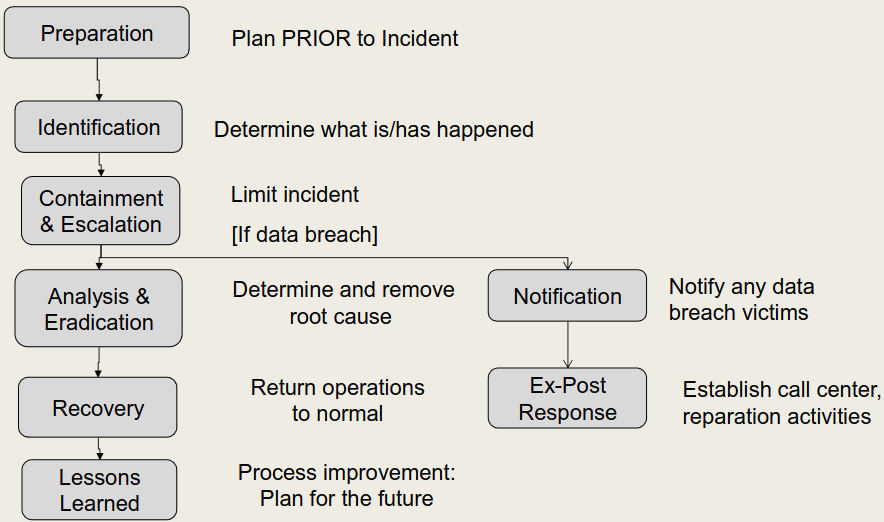
\includegraphics[width=0.45\columnwidth]{images/incident_response.png}
   \caption{Reaction on the Target System}
   \label{fig:incident_response}
\end{figure}

\begin{itemize}
   
   \item \textbf{Containment}
   
   The main purpose of containment is to contain the
   damage and prevent further damage.
   The earlier intrusions are
   detected, the sooner they can be contained.
   \item \textbf{Eradication}
   
   Removes the threat and restoring affected systems
   to their previous state while minimizing data loss.
   It should remove
   malicious content and ensure the affected systems are completely
   clean but preserve evidence for later prosecution
   \item \textbf{Recovery}
   
   Testing, monitoring, and validating systems before
   putting them back into production to assure they are not re-infected or compromised (backup fundamentals, 3-2-1 rule )
   \item \textbf{Lessons Learned}
   
   It gives organizations the opportunity to update
   the target system to prevent future intrusion and to understand
   how to improve intrusion management.
\end{itemize}

\subsection{Containment}
\labelitemize{
   \textit{Containment mechanisms}
}{

   \begin{enumerate}
      \item \textit{Host quarantine}
      
      Host quarantine prevents an infected host from communicating with other hosts;
      it is implemented via IP-level access control lists on routers or firewalls.
      
      \item \textit{String-matching}
      
      String-matching containment matches network traffic against signatures of known worms to drop associated packets.
      
      \item \textit{Connection throttling.}
      
      Connection throttling proactively limits the rate of all outgoing
      connections made by a machine and thereby slowing {---}not stopping{---}
      worm spreading. 
      It was proposed in a host context, but it can be applied to the network level as well.
   
   \end{enumerate}
}

\subsection{Forensics}
\begin{figure}[htbp]
   \centering
   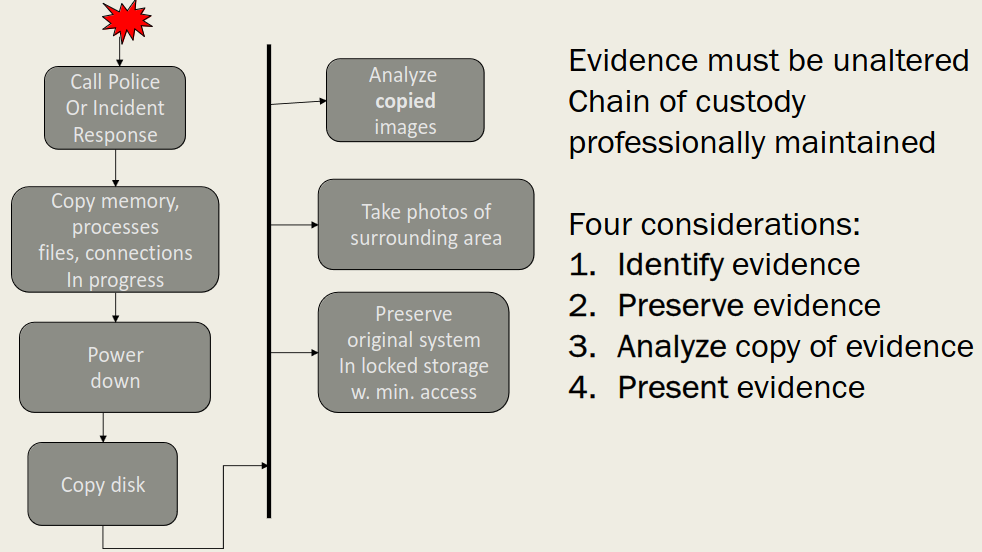
\includegraphics{images/intrusion_forensics.png}
   \caption{Intrusion forensics}
   \label{fig:intrusion_forensics}
\end{figure}

Note that proper \textbf{logging} allows easier eradication and forensics analysis,
where \textit{"proper"} indicates a log file which records at least any of
\begin{itemize}
   \item Login attempt
   \item Failed login
   \item Access to critical resources
   \item Anomalous messages (\texttt{Snort} log facility)
\end{itemize}
Besides, the log file should also be protected to guarantee its \textbf{integrity}, otherwise it's useless.
\begin{itemize}
   \item Write once memory 
   \note{"paper-like"}
   \item Insert a sequence number to discover log manipulation
   \item Insertion in a record of a value that is a function of all the previous
   records 
   note{hash pointer or blockchain}
\end{itemize}

Lastly,
to be useful from a \textbf{forensics} point of view,
the log file should be structured so that it can be used to prosecute the attacker and be exploited as a \textbf{legal} source of evidence in an
investigation and possibly chain of custody.

\subsection{Compromise recording}
Attackers who infect your system using \textit{ransomwares} stole your data and then encrypt it on your local disks,
then they ask for a ransom in order to have the data back.
A few years ago,
backups were very effective as a countermeasures to such attacks,
and they still are a key point to achieve \textit{resilience}\footnote{i.e. put the system back on},
there is still the problem that the stolen data may contain sensitive or personal information,
which should not be made public.

\subsection{Security vs Debugging logging}
When logging for \textbf{security} defending the \textbf{integrity} of the log
from malicious manipulation is \textit{fundamental}.
If the integrity of a log for security is not assured, then the log is useless.

If logging is performed for debugging {---} or more generally to improve performance, correctness, etc.{---} instead,
integrity is not so crucial. 

The difference between a sequence of blocks and a blockchain is a good example of the difference between collect for debugging and collect for security.

\section{Attribution}
\textbf{Attribution}, i.e. tracking and identifying the perpetrator of an intrusion results in a
whole picture of the intrusions to enhance cybersecurity,
besides,
attribution can also improve the evaluation of the intrusion impact and
increase the investment in countermeasures.

The information to attribute an intrusion are:
\begin{itemize}
   \item Tools used
   \item Behaviors of the threat agent (to improve detection of future intrusions)
   \item The attack infrastructure
   \item Shared code
   \item The information collected in the intrusion (log + honeynet)
\end{itemize}
Attribution typically takes a long time and it may provide
\begin{itemize}
   \item Information to eradicate the intrusion
   \item No immediate value to containing an intrusion
   \item No evidence for a court of law
\end{itemize}